\documentclass[12pt]{article}
\newcommand*{\ThesisPath}{/Users/gleb/software/gm2code/thesis} % define commands from the thesis  and imports 
\input{\ThesisPath/MainPackages} % Packages, package configurations, and most settings:
\input{\ThesisPath/Commands} % Sets up links and commands 
\graphicspath{{fig/}}

\def\Title#1{\begin{center} {\Large {\bf #1} } \end{center}}

\begin{document}


\Title{Tracker EDM analysis note: \\ A measurement of the longitudinal magnetic field in \R1}

\bigskip\bigskip

%+\addtocontents{toc}{{\it D. Reggiano}}
%+\label{ReggianoStart}
\thispagestyle{empty}
\begin{raggedright}  
Gleb Lukicov$\,^{a,1}$\\
{\it $^{\mathrm{a}}$ Department of Physics and Astronomy, University College London, UK} \\
{ $^{1}$ g.lukicov@ucl.ac.uk}
\bigskip\bigskip
\end{raggedright}

\begin{center}
\today
\end{center}

\null\vspace{\fill}
\begin{abstract}
This document briefly outlines the methodology of the longitudinal magnetic field, $B_z$, measurement using the tracker data in \R1. The final results for the systematic uncertainty on $\omega_a$ due to $B_z$ are presented, and are found to be: $0 \ \mathrm{ppm} < \frac{\Delta \omega_a}{\omega_a} < 4  \ \mathrm{ppm} $.
\end{abstract}
\vspace{\fill}

\tableofcontents

\clearpage
\thispagestyle{plain}

\section{Introduction}
A presence of a longitudinal field, $B_z$, tilts the precession plane of the muon, as shown in \cref{fig:mf_tilt}, and modifies~\cite{Bill} the observed precession frequency according to 
\begin{equation}
  \omega_a= a_{\mu}\frac{e}{m_{\mu}}B \rightarrow \frac{e}{m_{\mu}}  \sqrt{ (a_{\mu}B_y)^2 + \left(\frac{(1+a_{\mu})B_z}{\gamma}\right)^2 }.
\end{equation}
It is therefore imperative to estimate this systematic effect on $\omega_a$.
\vspace{-0.2cm}
\begin{figure}[htpb]
    \centering
    \subfloat[]{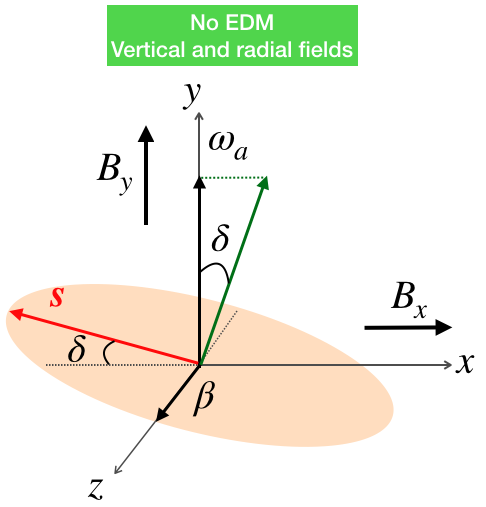
\includegraphics[width=0.45\linewidth]{mf_1.png}} 
    \subfloat[]{\hspace*{0.08\linewidth}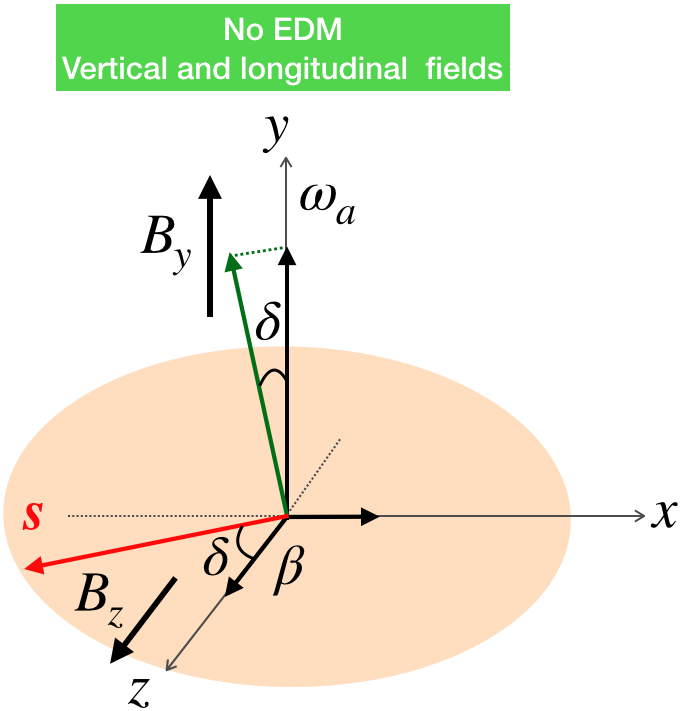
\includegraphics[width=0.45\linewidth]{mf_2.png}} 
    \vspace{-0.2cm}
    \caption{The tilt in the precession plane due to field components: a) radial ($B_x$) b) longitudinal ($B_z$). The momentum vector ($\beta$) is along the $z$-axis. The tilt due to the radial field - towards the centre of the ring - is analogous to an effect due to an EDM. The longitudinal field, however, would produce a tilt towards the direction of the stored beam, by an angle $\delta$.}
    \label{fig:mf_tilt}
\end{figure}

This tilt due to $B_z$ can be used in the measurement of the average vertical angle of muon decay as a function of time: an up-down oscillation in-phase with $\omega_a$ would be indicative of a longitudinal field.

\clearpage
\thispagestyle{plain}

\section{Methodology}
In this study, the measurement of the vertical angle, $\theta_y$, is coming from the tracking detector, where for each track a corresponding measurement of track time in a fill is available. This time is used to modulate data by the $g-2$ period, $T_{g-2}$, to remove any systematic effects that are not periodic with $T_{g-2}$ (e.g. VBO). This is analogous to the method used in the BNL EDM analysis by M. Sossong~\cite{Sossong}. The remaining analysis steps also follow the Sossong's methodology closely, and are presented in detail in DocDB:22201~\cite{Gleb_docdb}. These steps include fitting data for the number oscillation
\begin{equation}
     N(t)=Ne^{-t/\tau}[1+A\cos(\omega_at+\phi)],
     \label{eq:N}
\end{equation}
using a constant value of \SI{1.439311}{\MHz} for $\omega_a$, as measured at the BNL $g-2$~\cite{BNL_AMM}. This is shown in~\cref{fig:s12_bz_1}. The value of $\phi$ from~\cref{eq:N} is then used in the fit to the vertical angle oscillation
\begin{equation}
    \theta(t) =  A_{\mathrm{B_z}}\cos(\omega_a t + \phi) + A_{\mathrm{EDM}}\sin(\omega_a t + \phi) + c,
\end{equation}
where $A_{\mathrm{B_z}}$ is the amplitude due to the longitudinal magnetic field, $A_{\mathrm{EDM}}$ is the EDM amplitude, and $c$ is the overall offset. This is shown in~\cref{fig:s12_bz_2}. $A_{\mathrm{EDM}}$ is blinded with data, as discussed in DocDB:22201~\cite{Gleb_docdb}.

Parameter stability scans with fit start time, fit end time, momentum cuts, bin width, and a choice of $T_{g-2}$ (i.e. $\omega_a$) and $\phi$ are also presented in DocDB:22201~\cite{Gleb_docdb}, and are found to be stable.
\clearpage
\thispagestyle{plain} 

\begin{figure}[htpb]
    \centering
    \subfloat[]{\includegraphics[width=0.85\linewidth]{count_60h_S12.png}\label{fig:s12_bz_1}} \\ 
    \subfloat[]{\includegraphics[width=0.85\linewidth]{bz_60h_S12.png}\label{fig:s12_bz_2}} 
    \vspace{-0.2cm}
    \caption{Fitting results in the 60h dataset for S12: a) number oscillation, and b) average vertical angle oscillation.}
    \label{fig:s12_bz}
\end{figure}


\clearpage
\thispagestyle{plain}
\section{Results}
The observed (i.e. fitted) amplitudes of the vertical angle oscillation due to $B_z$ (i.e. $A_{\mathrm{B_z}}$) from all the four \R1 datasets are presented in \cref{fig:bz}.

\begin{figure}[htpb]
    \centering
    \subfloat[]{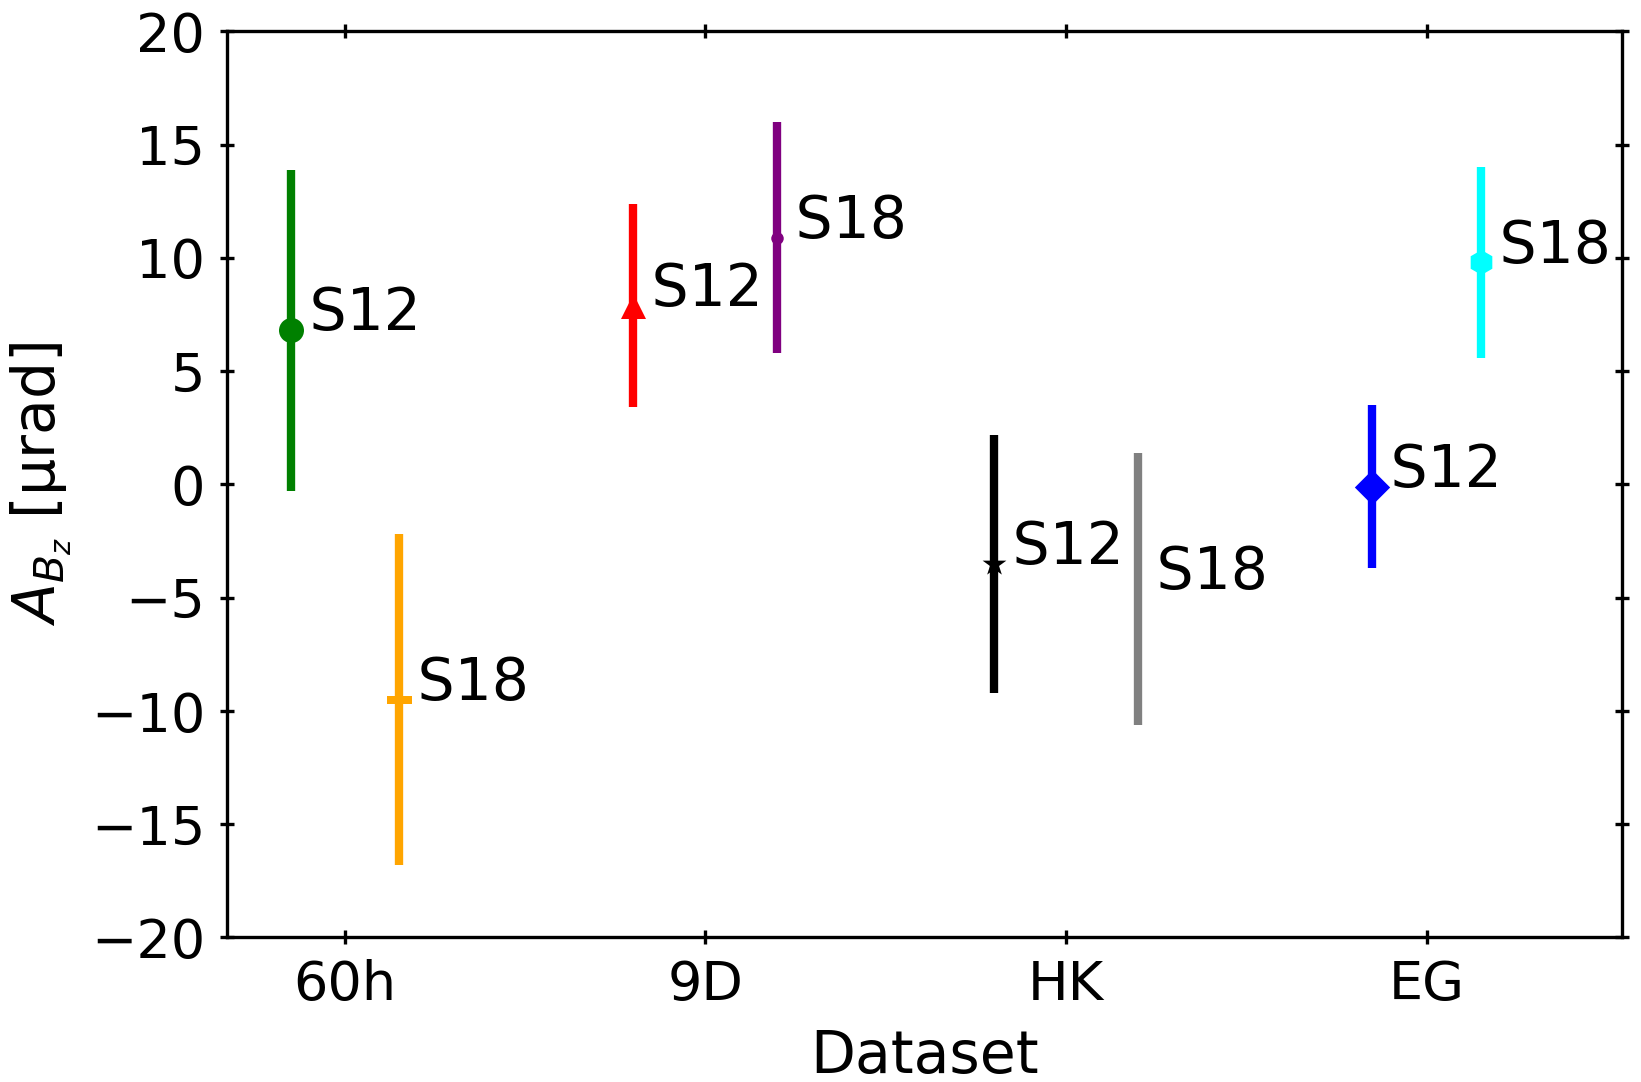
\includegraphics[width=0.65\linewidth]{s12S18_sum_bz.png}\label{fig:bz_1}} \\  
    \subfloat[]{\hspace{1cm}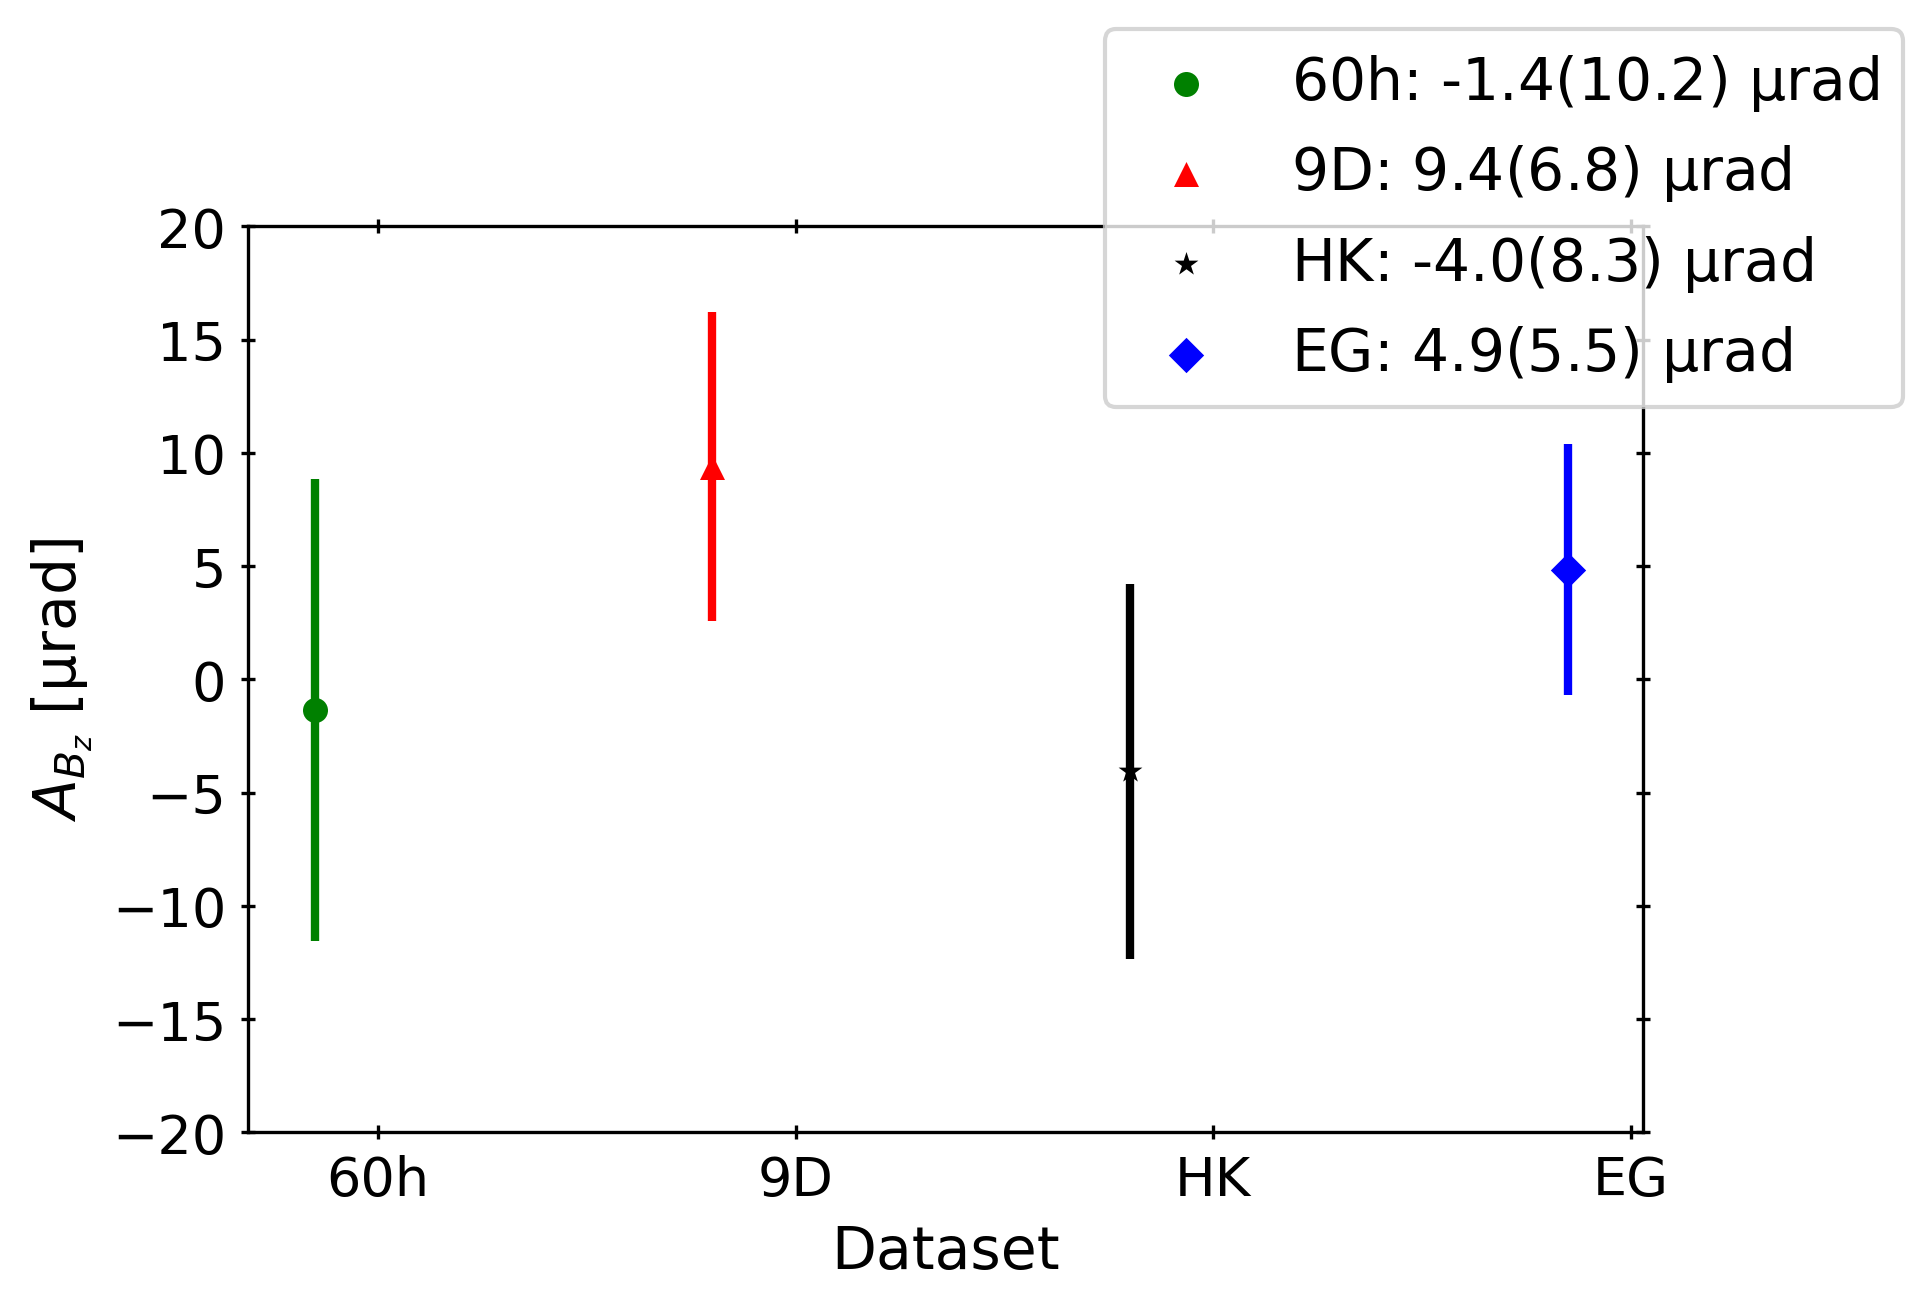
\includegraphics[width=0.75\linewidth]{sum_bz.png}\label{fig:bz_2}} 
    \vspace{-0.2cm}
    \caption{Fitting results in all \R1 datasets: a) S12 and S18 separately, and b) mean of the two stations. The individual fit results are summarised in DocDB:22201~\cite{Gleb_docdb}.}
    \label{fig:bz}
\end{figure}

\clearpage
\thispagestyle{plain}
Joe has posted a great and comprehensive note~\cite{Joe_Gleb}, which deals with a conversion from an observed amplitude to an estimated value of $B_z$. The conversion steps are as follows. Asymmetry term, $A=0.1$, is connecting the observed amplitude ($A_{\mathrm{B_z}}$) with the actual precession plane tilt in the lab frame ($\delta '$)
\begin{equation}
    A_{B_z}=0.1\delta '.
\end{equation}
Asymmetry is accounting for the fact that not all positrons are emitted in the direction of polarisation vector~\cite{Joe_Gleb}. Given that the muon motion is along $z$ (c.f.~\cref{fig:mf_tilt}), there is no Lorentz boost in this direction. Therefore, the estimate of $B_z$ is directly available from the measured angle in the lab frame, after the asymmetry term is taken into account. Hence, 
\begin{equation}
    \delta ' = \tan(\frac{B_z}{B_y})  \approx \frac{B_z}{B_y}.
    \label{eq:bz_ppm}
\end{equation}
Finally, the corresponding systematic uncertainty on $\omega_a$ can be estimated using the formula in Bill's note~\cite{Bill}
\begin{equation}
    \frac{\Delta \omega_a}{\omega_a} = \frac{1}{2}\left(\frac{(1+a_{\mu})}{a_{\mu}\gamma}\frac{B_z}{B_y}\right)^2.
    \label{eq:omega_ppm}
\end{equation}
The final results of the application of~\cref{eq:bz_ppm,eq:omega_ppm} to \R1 vertical angle oscillation is given in~\cref{fig:felina}.

\clearpage
\thispagestyle{plain} 

\begin{figure}[htpb]
    \centering
    \subfloat[]{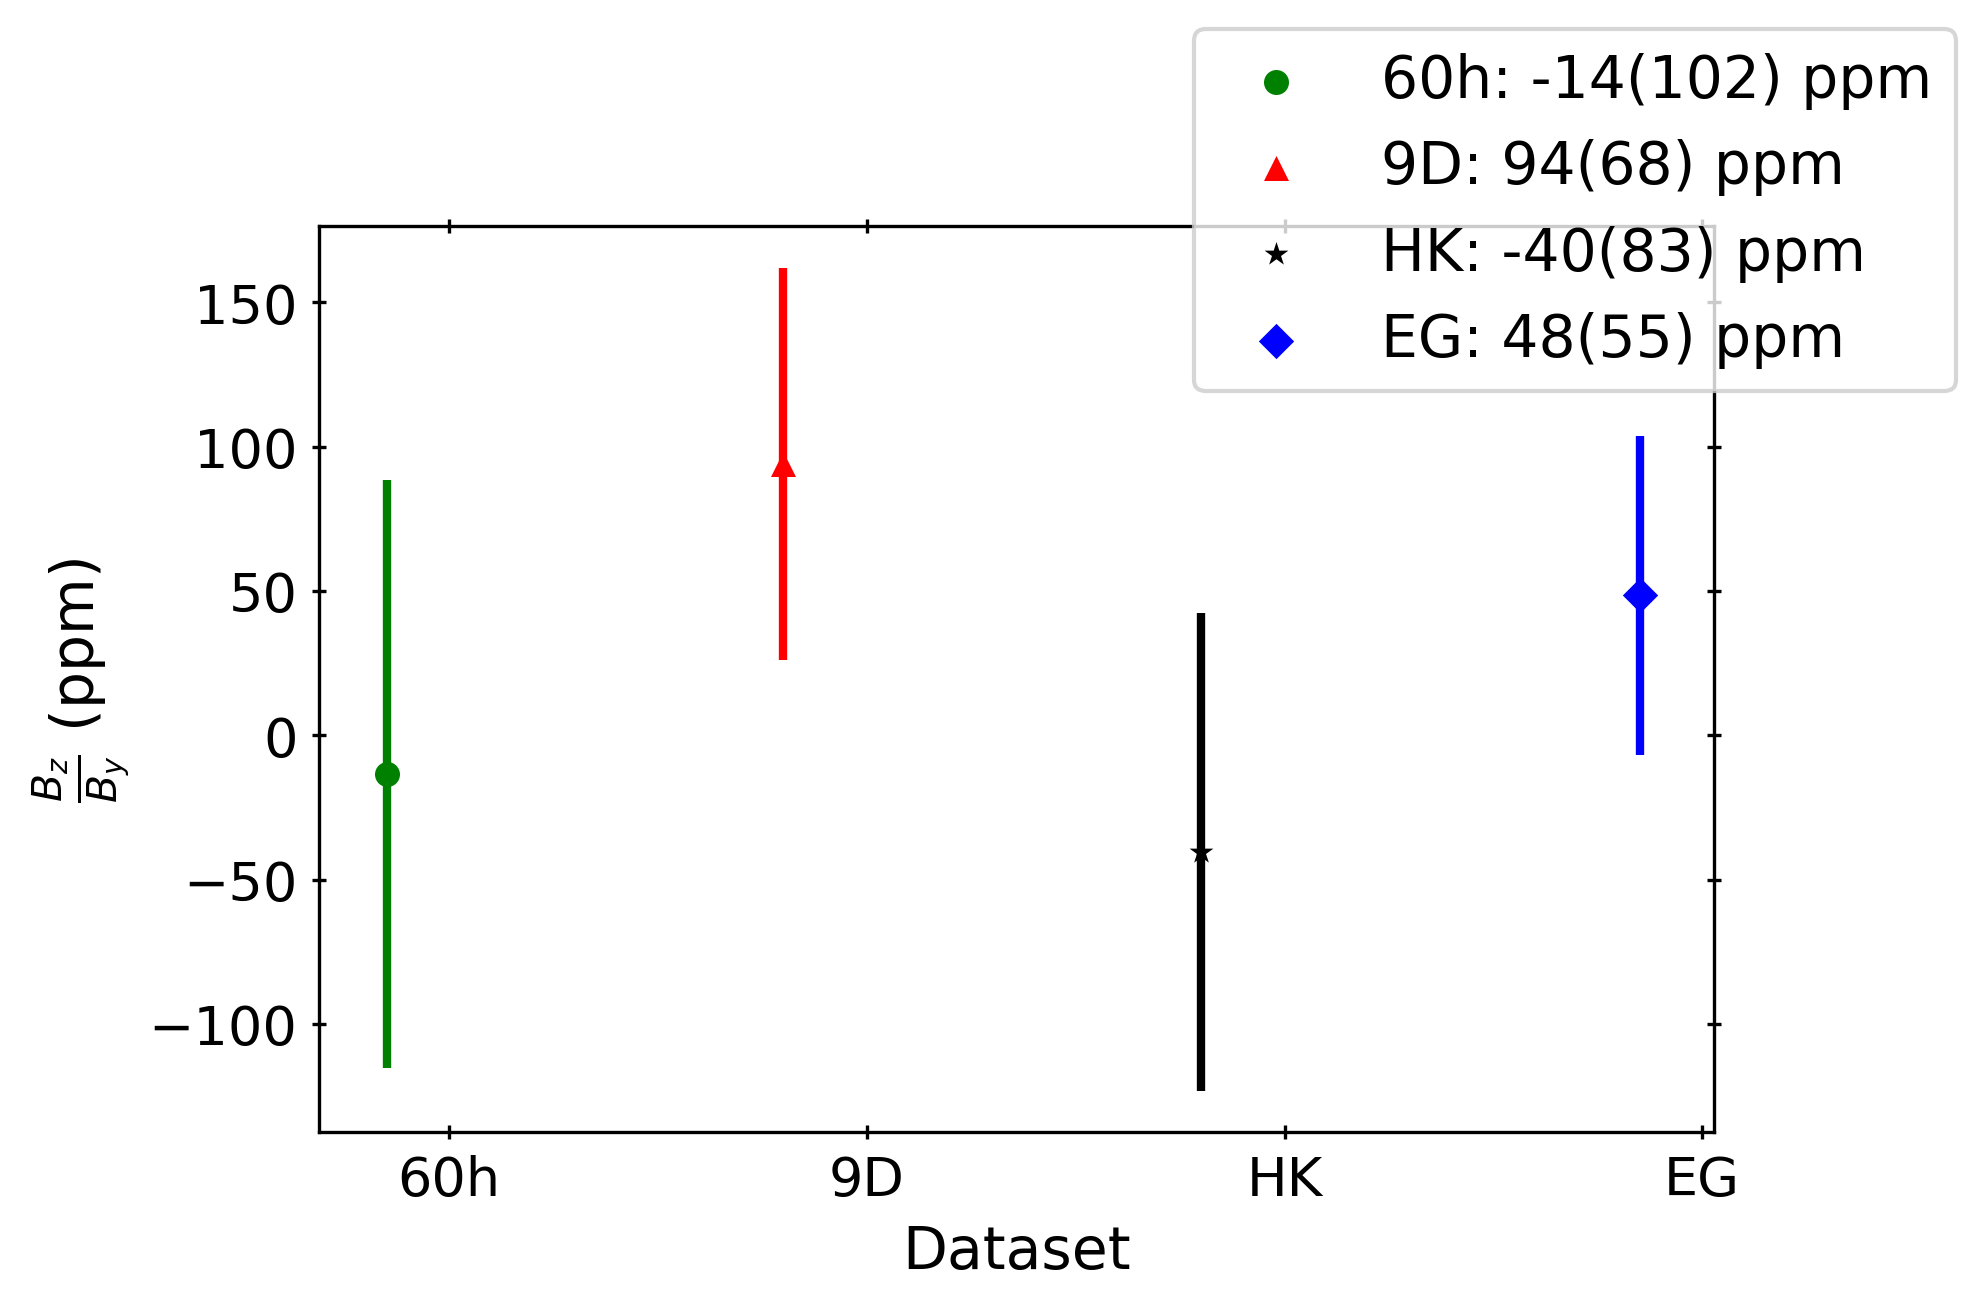
\includegraphics[width=0.75\linewidth]{ppm_bz.png}\label{fig:felina_1}} \\
    \subfloat[]{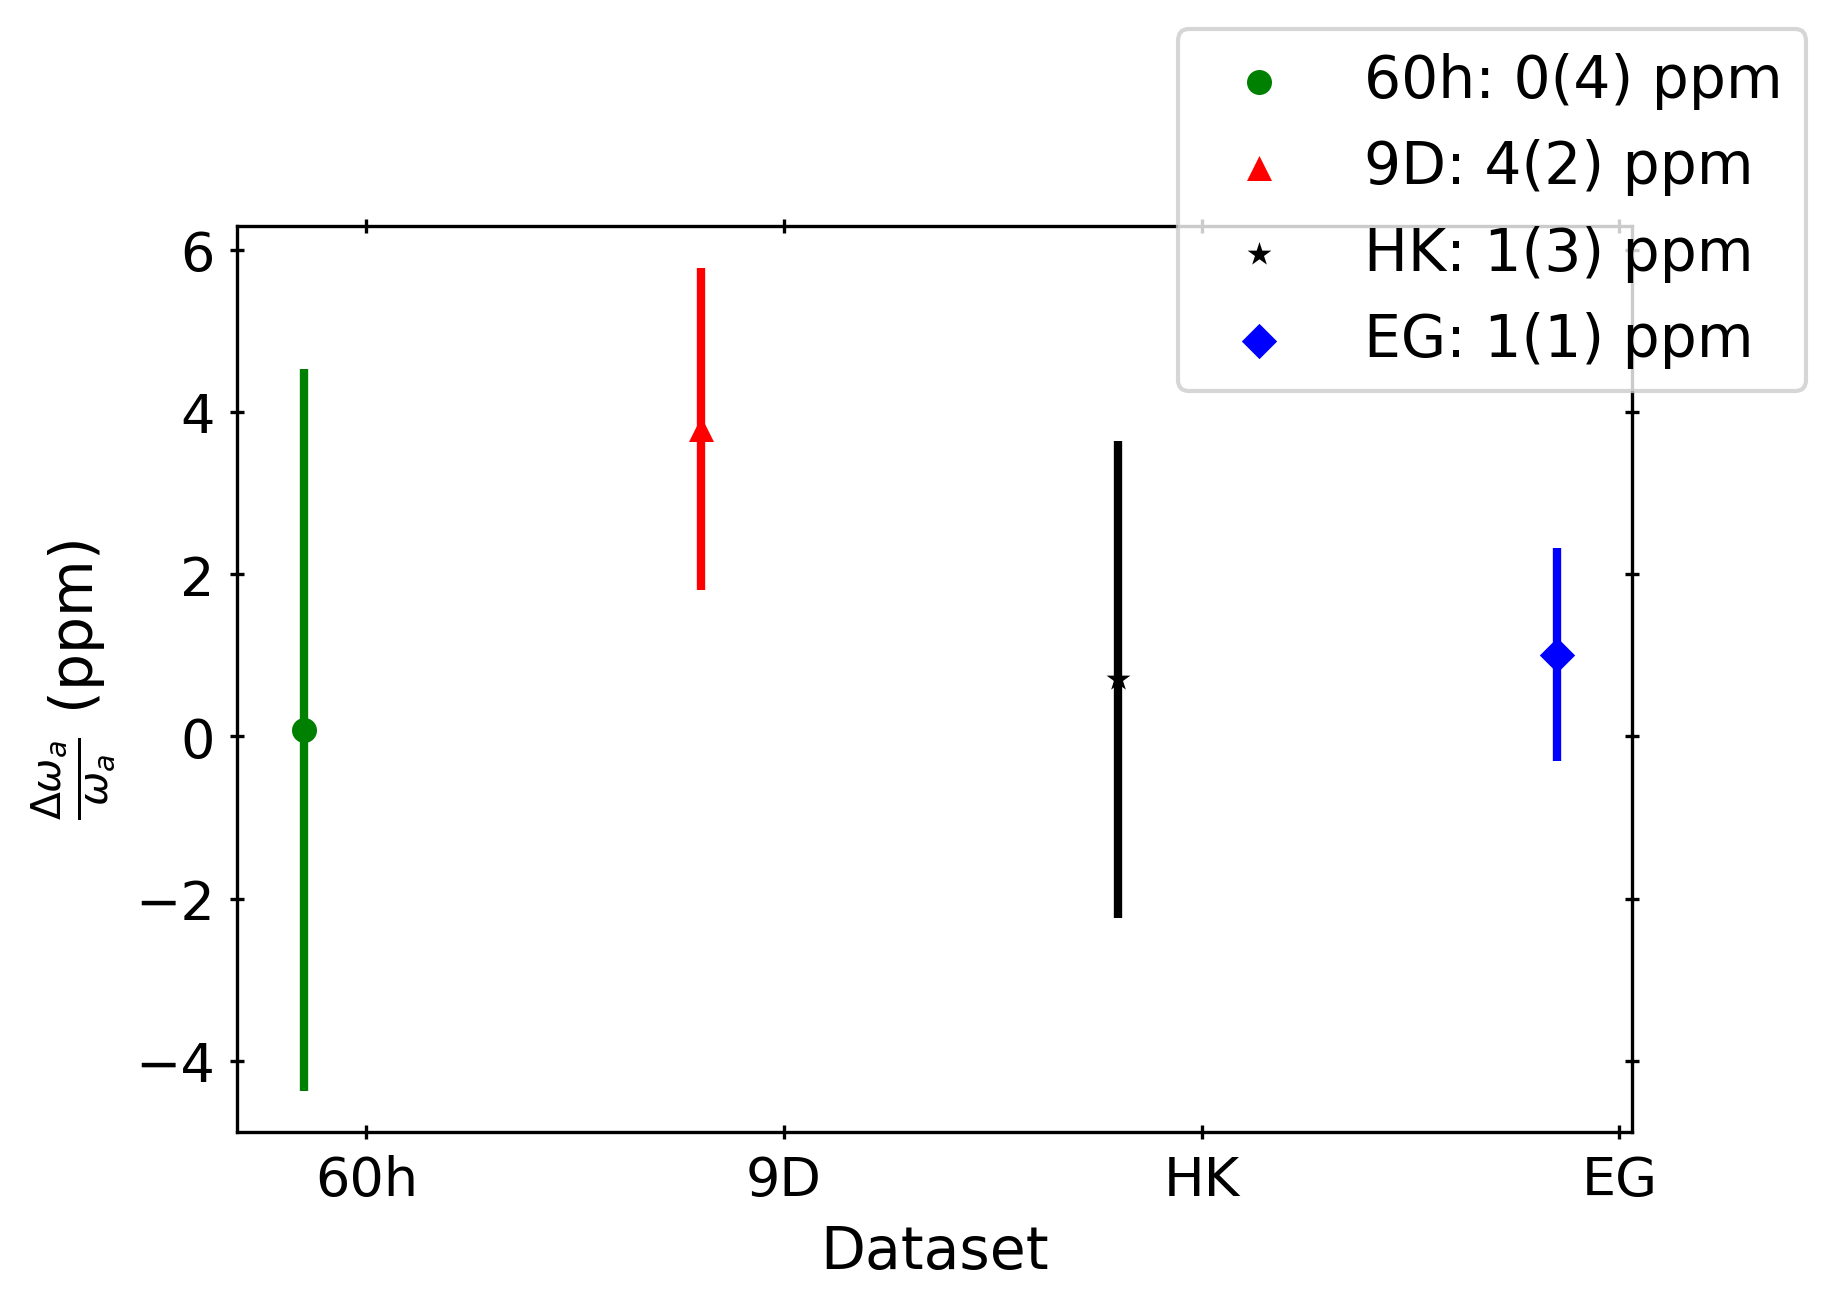
\includegraphics[width=0.7\linewidth]{ppm_omega.png}\label{fig:felina_2}} 
    \vspace{-0.2cm}
    \caption{\R1 systematic uncertainty results: a) $B_z$ in ppm and b) $\omega_a$ in ppm.}
    \label{fig:felina}
\end{figure}

Given the range of values in \cref{fig:felina_2}, the uncertainty spread on $\omega_a$ can be summarised as
\begin{equation}
    0 \ \mathrm{ppm} < \frac{\Delta \omega_a}{\omega_a} < 4  \ \mathrm{ppm}. 
\end{equation}

\clearpage
\thispagestyle{plain} 


\small
\bibliography{\ThesisPath/ref.bib} % Actually generates bibliography from ref.bib fle 
\normalsize

\def\Acknowledgements{
\setlength{\parskip}{0.3cm}\setlength{\parindent}{0.0cm}
     \bigskip\bigskip      {\Large {\bf Acknowledgements}} \bigskip}
\def\speaker#1{{\bf #1:}\ }
\def\endAcknowledgements{}
\Acknowledgements \\
I would like to express gratitude to Mark, Becky, Joe, James, Saskia, and Nick for their advice and guidance in this project. Also, I would like to thank the entire EDM group for their support and feedback.
\endAcknowledgements
 
\end{document}